\documentclass[11pt]{article}
\usepackage[letterpaper,margin=1in]{geometry}
\usepackage{amsmath,amssymb,bm}
\usepackage{graphicx}
\usepackage{booktabs}
\usepackage{xcolor}
\usepackage[hidelinks]{hyperref}
\setlength{\parindent}{0pt}
\setlength{\parskip}{0.7em}

\newcommand{\vocab}{\mathcal{V}}
\newcommand{\softmax}{\operatorname{softmax}}
\newcommand{\sigmoid}{\sigma}

\title{CS 224n Assignment 2: word2vec\\Written Solutions}
\author{}
\date{}

\begin{document}
\maketitle

\section*{1. Understanding word2vec}

\subsection*{(a) Cross-entropy form of the naive-softmax loss}
Because $\bm y$ is one-hot with $y_o=1$ and $y_w=0$ for $w\ne o$,
\[
-\sum_{w\in\vocab} y_w\log \hat y_w
=-\log \hat y_o
=-\log P(O=o\mid C=c)
=J_{\text{naive-softmax}}(\bm v_c,o,U).
\]

\subsection*{(b) Gradient with respect to the center vector}
Let $\bm z=U^\top\bm v_c$ and $\hat{\bm y}=\softmax(\bm z)$. The softmax cross-entropy derivative is
$\partial J/\partial\bm z=\hat{\bm y}-\bm y$. Since $\partial\bm z/\partial\bm v_c=U^\top$,
\[
\boxed{\frac{\partial J_{\text{naive-softmax}}}{\partial \bm v_c}
=U(\hat{\bm y}-\bm y).}
\]

\subsection*{(c) Gradients with respect to the outside vectors}
For each vocabulary word $w$,
\[
\frac{\partial J_{\text{naive-softmax}}}{\partial \bm u_w}
=(\hat y_w-y_w)\bm v_c.
\]
Equivalently,
\[
\boxed{
\frac{\partial J}{\partial \bm u_w}=
\begin{cases}
(\hat y_o-1)\bm v_c, & w=o,\\
\hat y_w\bm v_c, & w\ne o.
\end{cases}}
\]

\subsection*{(d) Derivative of the sigmoid}
For every component $x_i$ of a vector $\bm x$,
\[
\boxed{\frac{\partial\sigmoid(x_i)}{\partial x_i}
=\sigmoid(x_i)\bigl(1-\sigmoid(x_i)\bigr).}
\]
Thus the elementwise derivative is
$\sigmoid(\bm x)\odot(\bm 1-\sigmoid(\bm x))$; the full Jacobian is the diagonal matrix containing these values.

\subsection*{(e) Negative sampling gradients}
Write $a_o=\bm u_o^\top\bm v_c$ and $a_k=\bm u_k^\top\bm v_c$. Using
$\frac{d}{dx}[-\log\sigmoid(x)]=\sigmoid(x)-1$ and
$\frac{d}{dx}[-\log\sigmoid(-x)]=\sigmoid(x)$ gives
\[
\boxed{
\frac{\partial J_{\text{neg-sample}}}{\partial \bm v_c}
=(\sigmoid(a_o)-1)\bm u_o
+\sum_{k=1}^{K}\sigmoid(a_k)\bm u_k,}
\]
\[
\boxed{
\frac{\partial J_{\text{neg-sample}}}{\partial \bm u_o}
=(\sigmoid(a_o)-1)\bm v_c,}
\qquad
\boxed{
\frac{\partial J_{\text{neg-sample}}}{\partial \bm u_k}
=\sigmoid(a_k)\bm v_c.}
\]
If a negative word is sampled more than once, its contributions are added. Negative sampling is more efficient because it updates only the true outside word and $K$ sampled words, rather than computing and updating scores for the entire vocabulary.

\subsection*{(f) Skip-gram gradients over a context window}
Let $S=\{j:-m\le j\le m,\ j\ne0\}$. Since the skip-gram objective is a sum over outside words,
\[
\boxed{
\frac{\partial J_{\text{skip-gram}}}{\partial U}
=\sum_{j\in S}\frac{\partial J(\bm v_c,w_{t+j},U)}{\partial U},}
\]
\[
\boxed{
\frac{\partial J_{\text{skip-gram}}}{\partial \bm v_c}
=\sum_{j\in S}\frac{\partial J(\bm v_c,w_{t+j},U)}{\partial \bm v_c},}
\]
and, for every center-word vector $\bm v_w$ with $w\ne c$,
\[
\boxed{
\frac{\partial J_{\text{skip-gram}}}{\partial \bm v_w}=\bm 0.}
\]

\clearpage
\section*{2(c). Trained word vectors}
\begin{figure}[h!]
  \centering
  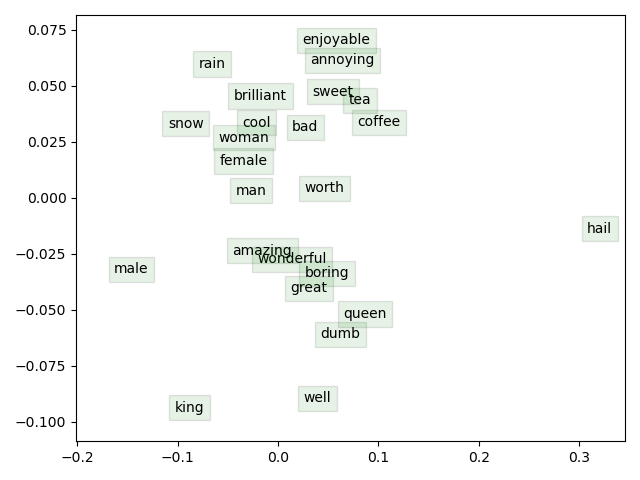
\includegraphics[width=0.82\textwidth]{word_vectors.png}
  \caption{Two-dimensional projection of the word vectors learned from the Stanford Sentiment Treebank.}
\end{figure}

The projection shows meaningful local relationships: ``coffee'' is close to ``tea,'' ``woman'' is close to ``female'' and ``man,'' and ``great,'' ``wonderful,'' and ``amazing'' form a compact group. Some expected relationships are imperfect: ``rain'' is nearer to ``snow'' than to ``hail,'' while sentiment words such as ``enjoyable''/``annoying'' and ``wonderful''/``boring'' are not cleanly separated. This noise is reasonable because the vectors are trained on a modest corpus and a two-dimensional projection cannot preserve every relationship in the original ten-dimensional space.

\end{document}
